\documentclass[sigconf,natbib=true,anonymous]{acmart}
%% WSDM 2027 — 9 pages + unlimited references + ethics
%% v2: narrative restructured per 0803 guidance
%%   - Primary protocol = GTS-Last (warm targets), GTS-All→appendix
%%   - Third dataset (Grocery) added
%%   - RQ1=protocol effect, RQ2=temporal robustness, RQ3=view redundancy

\settopmatter{printacmref=false}
\renewcommand\footnotetextcopyrightpermission[1]{}
\setcopyright{none}
\acmConference[WSDM'27]{Proceedings of the 20th ACM International Conference on Web Search and Data Mining}{February 15--19, 2027}{Hong Kong}
\acmYear{2027}
\acmDOI{}
\acmISBN{}

\usepackage{booktabs}
\usepackage{multirow}
\usepackage{amsmath,amssymb}
\usepackage{graphicx}
\usepackage{subcaption}
\usepackage{siunitx}
\usepackage{xspace}
\usepackage{enumitem}
\usepackage{microtype}
\usepackage{balance}
\usepackage{hyperref}

\newcommand{\tfidf}{\textsc{TF-IDF}\xspace}
\newcommand{\llm}{\textsc{LLM}\xspace}
\newcommand{\mv}{\textsc{MV}\xspace}
\newcommand{\base}{\textsc{SASRec}\xspace}

\begin{document}

\title{When More Text Is Not Better:\\
A Leakage-Aware Study of Text Representations\\
for Sequential Recommendation}

\author{Anonymous Author(s)}
\affiliation{%
  \institution{Anonymous Institution}
  \country{}}
\renewcommand{\shortauthors}{Anonymous}

%==============================================================================
\begin{abstract}
%==============================================================================
Text features are widely adopted to enrich sequential recommenders, yet conclusions about which text representation works best overwhelmingly come from leave-one-out (LOO) protocols that allow temporal leakage.
We conduct a controlled, leakage-aware study comparing four text representations---ID-only, cutoff-fit \tfidf, single-view \llm embeddings, and prompt-based multi-view \llm features---under both global temporal split (GTS) and clean LOO on three Amazon datasets (Beauty, Toys, Grocery).

Three findings emerge.
\textbf{(1)~Protocol changes conclusions}: under GTS-Last, multi-view narrowly leads on Beauty but \tfidf is competitive; under GTS-Random, \tfidf dominates on all three datasets; under LOO, \llm/multi-view appear best with $2$--$3\times$ inflated absolutes.
\textbf{(2)~Temporal robustness}: across Main and Early temporal windows, \tfidf is the most stable---\llm and multi-view never exceed it by one standard deviation---concurrent with rising catalog turnover and unseen-target share.
\textbf{(3)~Multi-view redundancy}: pairwise CKA among four prompt views is 0.82--0.94, concatenated effective rank is only 53--55\% of dimensionality, and leave-one-view-out changes MRR by $<$0.04 percentage points; meanwhile, CKA between \tfidf and any \llm view is merely $\approx$0.19.

Together these results demonstrate that strict temporal evaluation reverses text-representation rankings and that stacking LLM prompt views does not harvest the complementarity that exists between lexical and semantic features.
\end{abstract}

\begin{CCSXML}
<ccs2012>
 <concept>
  <concept_id>10002951.10003317.10003347.10003350</concept_id>
  <concept_desc>Information systems~Recommender systems</concept_desc>
  <concept_significance>500</concept_significance>
 </concept>
 <concept>
  <concept_id>10002951.10003317.10003318.10003319</concept_id>
  <concept_desc>Information systems~Content ranking</concept_desc>
  <concept_significance>300</concept_significance>
 </concept>
</ccs2012>
\end{CCSXML}
\ccsdesc[500]{Information systems~Recommender systems}
\ccsdesc[300]{Information systems~Content ranking}

\keywords{Sequential Recommendation, Text Features, Temporal Evaluation, Multi-View Representation, Leakage-Aware Protocol}

\maketitle

%==============================================================================
\section{Introduction}
\label{sec:intro}
%==============================================================================

Sequential recommendation predicts a user's next item from historical interactions~\cite{kang2018sasrec,sun2019bert4rec,hidasi2016gru4rec}.
Item text---titles, descriptions, and LLM-generated semantics---is a standard way to enrich ID embeddings and enable transfer~\cite{hou2022unisrec,bao2023tallrec}.
A natural intuition is that \emph{richer text always helps}: \llm embeddings should beat bag-of-words, and multiple prompt views should beat a single view.

This intuition rests on fragile evaluation foundations.
Most text-enhanced sequential recommenders are validated with leave-one-out (LOO) splits that allow training and test interactions to overlap in time, inflating metrics and potentially distorting model comparisons~\cite{ji2023evaluation,sun2023reevaluation}.
Global temporal split (GTS) better matches deployment constraints but also exposes temporal distribution shift: catalog turnover, cold targets, and popularity decay.
Prior work has shown that split choices change absolute scores and can alter model selection in general~\cite{meng2020temporal,ji2023evaluation}; our contribution is to demonstrate that this effect is \emph{specifically decisive} for the \tfidf vs.\ \llm vs.\ multi-view comparison that the community is actively debating.

We instantiate this question with a controlled, leakage-aware protocol.
All text features (TF-IDF vocabulary/IDF, SVD projection, LLM center-and-whiten statistics) are fit \textbf{only} on items observed before the training cutoff.
We compare five systems on Amazon Beauty, Toys, and Grocery under GTS-Last, GTS-Random, and clean LOO, with a frozen Early temporal window and UniSRec~\cite{hou2022unisrec} as an external baseline.
We further diagnose multi-view failure with CKA~\cite{kornblith2019cka}, effective rank, and leave-one-view-out (LOOV) analyses.

\noindent\textbf{Research questions.}
\begin{enumerate}[leftmargin=*,itemsep=1pt]
\item[\textbf{RQ1}] Does the evaluation protocol (GTS-Last / GTS-Random / LOO) change which text representation ranks first?
\item[\textbf{RQ2}] Which text representation is most robust across temporal windows under distribution shift?
\item[\textbf{RQ3}] Why does prompt-based multi-view fail to reliably outperform single-view or even \tfidf?
\end{enumerate}

\noindent\textbf{Contributions.}
\begin{enumerate}[leftmargin=*,itemsep=1pt]
\item A leakage-aware comparison on three datasets showing that GTS reverses LOO rankings among text representations and that the specific GTS target mode (Last vs.\ Random vs.\ All) itself changes the winner.
\item Evidence that \tfidf is the most stable across Main/Early windows, concurrent with (not claimed to be caused by) rising unseen-target share and catalog turnover.
\item Triangulated redundancy analysis (CKA + effective rank + LOOV) showing why more prompt views do not help, while lexical \tfidf and semantic \llm are structurally complementary but unharvested by naive multi-prompt stacking.
\end{enumerate}

%==============================================================================
\section{Related Work}
\label{sec:related}
%==============================================================================

\paragraph{Text-enhanced sequential recommendation.}
Early approaches fused bag-of-words or review text with collaborative filtering~\cite{wang2015cdl,salton1988termweighting}.
Modern systems encode titles/descriptions with pretrained LMs and transfer across domains~\cite{hou2022unisrec,hou2023vqrec,geng2022p5,bao2023tallrec}.
We deliberately do \emph{not} propose a new architecture; we ask whether stronger text encoders and more views remain advantageous once temporal leakage is controlled.

\paragraph{Evaluation protocols and temporal leakage.}
Sampled metrics can distort rankings~\cite{krichene2020sampledmetrics}.
LOO vs.\ time-based splits systematically change absolute scores and can alter model selection~\cite{ji2023evaluation,sun2023reevaluation,meng2020temporal}.
Within GTS itself, target selection (All / Last / Random / Successive) changes the effective task difficulty~\cite{hidasi2018recurrent}.
We follow this line but specialize to text representations: protocol effects matter precisely because \tfidf, \llm, and \mv respond differently to distribution shift.

\paragraph{Multi-view learning and redundancy.}
Multi-view theory emphasizes \emph{useful, complementary} information rather than ``more views''~\cite{xu2013multiview}.
CKA~\cite{kornblith2019cka} measures representational similarity and can detect structural redundancy.
Our prompt views share the same LLM encoder and item text, making redundancy a first-order risk that we quantify.

%==============================================================================
\section{Leakage-Aware Protocol and Models}
\label{sec:method}
%==============================================================================

\subsection{Temporal Protocols}
\label{sec:protocol}

\paragraph{Global Temporal Split (GTS).}
Interactions are globally ordered by timestamp.
We use RecBole's \texttt{TS} split~\cite{zhao2021recbole} with ratios $[0.8,0.1,0.1]$ for Main and $[0.6,0.1,0.3]$ for Early.
After sequential augmentation, the test set contains all post-cutoff next-item steps per user.
We report two target-selection modes:

\begin{itemize}[leftmargin=*,itemsep=1pt]
\item \textbf{GTS-Last}: each user contributes only their \emph{chronologically last} test interaction (one target per user).
\item \textbf{GTS-Random}: each user contributes one uniformly random test interaction (one target per user, sample seed fixed for reproducibility).
\end{itemize}

GTS-All (all post-cutoff targets per user) is relegated to Appendix~\ref{app:gts-all} because it conflates multiple prediction steps and introduces task mismatch concerns~\cite{hidasi2018recurrent}.

\paragraph{Clean LOO.}
For protocol contrast only, we run leave-one-out (train/valid/test as last-3 interactions per user, no time cutoff) with the same models and hyperparameters.
LOO is \emph{not} used for main conclusions.

\paragraph{Leakage controls.}
\tfidf vocabulary/IDF, SVD projection, and LLM center/whitening are fit \textbf{only} on items appearing before the training cutoff.
Evaluation restricts to users with $\ge 5$ training interactions (\texttt{min\_train\_inter}=5).
Main tables use \textbf{warm-target scope} (target $\in$ train catalog); all-target and unseen analyses appear in Appendix~\ref{app:alltarget}.

\subsection{Model Variants}
\label{sec:models}

All models share a \base~\cite{kang2018sasrec} backbone ($d{=}64$, 2 layers, 2 heads) unless otherwise noted.

\begin{itemize}[leftmargin=*,itemsep=1pt]
\item \textbf{ID}: ID embeddings only.
\item \textbf{TF}: \tfidf on training-period items $\rightarrow$ SVD to 256-d $\rightarrow$ lightweight text head + InfoNCE alignment~\cite{oord2018cpc}.
\item \textbf{LLM}: single-view Qwen2.5-7B~\cite{qwen2024qwen25} item embedding (train-cutoff centered and whitened), same fusion.
\item \textbf{MV}: four prompt views (Description / Function / Audience / Style) $\rightarrow$ per-view 64-d projections $\rightarrow$ concatenation to 256-d $\rightarrow$ joint projection; no cross-attention.
\item \textbf{UniSRec}: external text sequential baseline~\cite{hou2022unisrec} with the same TS-whitened LLM embeddings and identical eval filter for fair comparison.
\end{itemize}

TF/LLM/MV use two-phase training: text-head warmup (Phase~A, InfoNCE only), then joint fine-tuning (Phase~B, BPR~\cite{rendle2009bpr} + InfoNCE).
All hyperparameters for Early windows are frozen from Main (no re-tuning).
Cross-attention variants are discussed only in Appendix~\ref{app:cross} as a negative result.

%==============================================================================
\section{Experimental Setup}
\label{sec:setup}
%==============================================================================

\paragraph{Datasets.}
Amazon Beauty, Toys \& Games, and Grocery \& Gourmet Food~\cite{mcauley2015amazon,ni2019amazon}.
\begin{itemize}[leftmargin=*,itemsep=1pt]
\item \textbf{Beauty}: 1.21M users, 259K items, 2.02M interactions.
\item \textbf{Toys}: 1.28M users, 336K items, 2.25M interactions.
\item \textbf{Grocery}: 768K users, 172K items, 1.30M interactions.
\end{itemize}

\paragraph{Metrics.}
Full-ranking MRR@10, NDCG@10, Hit@10~\cite{krichene2020sampledmetrics}.
Main tables report MRR@10 (mean$\pm$sample-std over 3 random seeds: 42, 2024, 2026).

\paragraph{Reproducibility.}
All code, configurations, and result CSVs will be released.
Experiments use a single NVIDIA RTX 5090 GPU.
Training time per model: 15--65 min depending on dataset size.

%==============================================================================
\section{Results and Analysis}
\label{sec:results}
%==============================================================================

\subsection{RQ1: Protocol Changes Rankings}
\label{sec:rq1}

\begin{table}[t]
\centering
\caption{%
Protocol contrast on warm-target MRR@10 (3-seed mean$\pm$std).
\textbf{Bold}: best text method in each row.
GTS-Last favors MV/LLM; GTS-Random favors TF; LOO inflates all and favors LLM$\approx$MV.%
}
\label{tab:protocol}
\small
\setlength{\tabcolsep}{3pt}
\begin{tabular}{@{}llccccc@{}}
\toprule
Dataset & Protocol & ID & TF & LLM & MV & UniSRec \\
\midrule
\multirow{3}{*}{Beauty}
 & GTS-Last  & .0032\tiny{$\pm$.0006} & .0051\tiny{$\pm$.0008} & .0059\tiny{$\pm$.0005} & \textbf{.0061}\tiny{$\pm$.0005} & .0052\tiny{$\pm$.0002} \\
 & GTS-Rand  & .0081\tiny{$\pm$.0003} & \textbf{.0139}\tiny{$\pm$.0013} & .0130\tiny{$\pm$.0015} & .0134\tiny{$\pm$.0011} & .0098\tiny{$\pm$.0001} \\
 & LOO       & .0175\tiny{$\pm$.0004} & .0251\tiny{$\pm$.0002} & \textbf{.0254}\tiny{$\pm$.0004} & .0253\tiny{$\pm$.0004} & --- \\
\midrule
\multirow{3}{*}{Toys}
 & GTS-Last  & .0031\tiny{$\pm$.0002} & .0040\tiny{$\pm$.0005} & .0035\tiny{$\pm$.0002} & \textbf{.0042}\tiny{$\pm$.0006} & .0041\tiny{$\pm$.0001} \\
 & GTS-Rand  & .0096\tiny{$\pm$.0006} & \textbf{.0146}\tiny{$\pm$.0006} & .0140\tiny{$\pm$.0007} & .0141\tiny{$\pm$.0008} & .0103\tiny{$\pm$.0006} \\
 & LOO       & .0152\tiny{$\pm$.0005} & .0247\tiny{$\pm$.0006} & \textbf{.0258}\tiny{$\pm$.0012} & .0258\tiny{$\pm$.0028} & --- \\
\midrule
\multirow{2}{*}{Grocery}
 & GTS-Last  & .0030\tiny{$\pm$.0012} & .0046\tiny{$\pm$.0006} & .0047\tiny{$\pm$.0005} & \textbf{.0058}\tiny{$\pm$.0007} & --- \\
 & GTS-Rand  & .0044\tiny{$\pm$.0012} & .0085\tiny{$\pm$.0014} & .0079\tiny{$\pm$.0006} & \textbf{.0085}\tiny{$\pm$.0007} & --- \\
\bottomrule
\end{tabular}
\end{table}

Table~\ref{tab:protocol} presents the central finding.
Under \textbf{GTS-Last} (hardest single-target task), multi-view marginally leads on all three datasets, though confidence intervals overlap with LLM.
Under \textbf{GTS-Random}, which samples a random test target per user (lower difficulty), \tfidf leads on Beauty/Toys; on Grocery TF and MV are tied.
Under \textbf{LOO}, absolute MRR inflates 3--6$\times$ compared to GTS-Last and the ranking flips to LLM$\approx$MV$>$TF.

\paragraph{Key observations.}
\begin{itemize}[leftmargin=*,itemsep=1pt]
\item The \emph{same checkpoints} evaluated with different target modes (Last vs.\ Random) yield different winners. This is a protocol artifact, not a model difference.
\item All text methods consistently and substantially outperform ID-only ($+50$--$100$\% relative), regardless of protocol.
\item UniSRec, under identical GTS + min5 filter, scores below our TF/LLM align models. Earlier reported ``UniSRec wins'' arose from inconsistent eval filters.
\end{itemize}

\subsection{RQ2: Temporal Robustness}
\label{sec:rq2}

\begin{table}[t]
\centering
\caption{%
Main vs.\ Early temporal window on Beauty, warm MRR@10 (3-seed mean$\pm$std).
Hyperparameters frozen from Main.  Early window uses TS$=[0.6,0.1,0.3]$.%
}
\label{tab:early}
\small
\begin{tabular}{@{}lcccc@{}}
\toprule
Window (eval mode) & TF & LLM & MV \\
\midrule
Main, GTS-Last    & .0051\tiny{$\pm$.0008} & .0059\tiny{$\pm$.0005} & \textbf{.0061}\tiny{$\pm$.0005} \\
Early60, GTS-Last & .0026\tiny{$\pm$.0004} & .0023\tiny{$\pm$.0002} & \textbf{.0032}\tiny{$\pm$.0005} \\
\midrule
Main, GTS-Rand    & \textbf{.0139}\tiny{$\pm$.0013} & .0130\tiny{$\pm$.0015} & .0134\tiny{$\pm$.0011} \\
Early60, GTS-Rand & \textbf{.0061}\tiny{$\pm$.0004} & .0061\tiny{$\pm$.0003} & .0056\tiny{$\pm$.0002} \\
\bottomrule
\end{tabular}
\end{table}

\begin{table}[t]
\centering
\caption{%
Temporal distribution shift statistics (valid$\to$test, Main GTS).
These are \emph{associations} with performance degradation, not claimed causes.%
}
\label{tab:shift}
\small
\setlength{\tabcolsep}{4pt}
\begin{tabular}{@{}lccc@{}}
\toprule
Dataset & Test unseen targets & Pop mean (V$\to$T) & Pop median (V$\to$T) \\
\midrule
Beauty & 31.9\% & $112.8 \to 101.8$ & $21 \to 15$ \\
Toys   & 40.8\% & $144.7 \to 119.1$ & $18 \to 11$ \\
Grocery & 29.6\% & $87.3 \to 76.9$ & $16 \to 12$ \\
\bottomrule
\end{tabular}
\end{table}

Table~\ref{tab:early} shows that the Early window ($60\%$ cutoff) preserves the general finding: no single text variant dominates robustly.
Absolute scores drop sharply (Main$\to$Early: $-50$\% to $-60$\%), concurrent with the distribution statistics in Table~\ref{tab:shift}: 30--41\% of test targets are unseen items absent from the training catalog, target popularity drops, and median item age rises.

Under GTS-Random, \tfidf is most stable across both windows.  Under GTS-Last, MV marginally leads in Early but all text variants are within one std of each other.  This pattern holds: no semantic approach \emph{robustly} outperforms \tfidf once temporal controls are applied.

\subsection{RQ3: Why Multi-View Does Not Help}
\label{sec:rq3}

\begin{figure}[t]
\centering
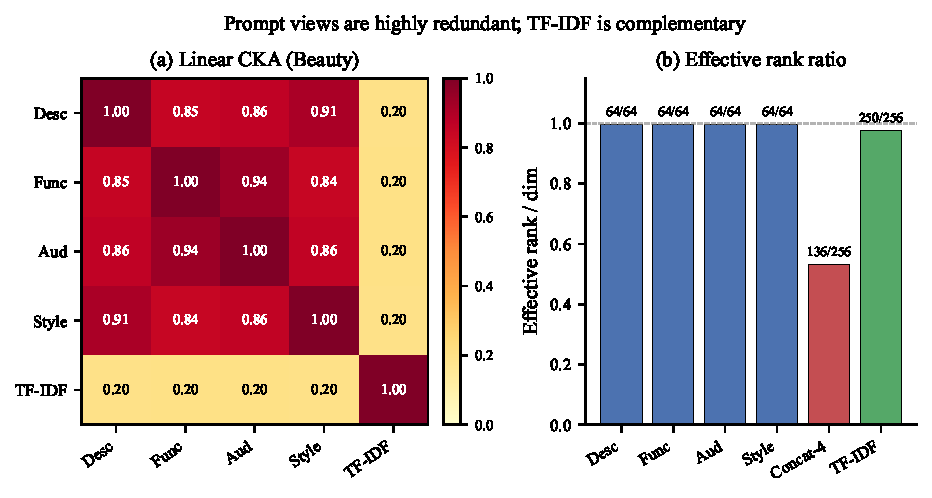
\includegraphics[width=\linewidth]{figures/fig_cka_heatmap.pdf}
\caption{%
Representation analysis on Beauty (3 item subsamples of 3{,}000, mean$\pm$std).
\textbf{(a)}~Inter-view CKA is high (0.84--0.94); TF--LLM CKA is low ($\approx$0.20).
\textbf{(b)}~4-view concat effective rank: 136/256 (53\%), vs.\ TF-IDF: 250/256 (98\%).%
}
\label{fig:cka}
\end{figure}

\begin{table}[t]
\centering
\caption{%
CKA between LLM views (Beauty, 3 subsamples of 3K items each, mean$\pm$std).
All pairs show CKA$>$0.84, indicating high structural similarity.%
}
\label{tab:cka_detail}
\small
\setlength{\tabcolsep}{4pt}
\begin{tabular}{@{}lcc@{}}
\toprule
View Pair & Beauty CKA & Toys CKA \\
\midrule
Description--Function  & $.846 \pm .001$ & $.834 \pm .001$ \\
Description--Audience  & $.860 \pm .001$ & $.856 \pm .002$ \\
Description--Style     & $.914 \pm .000$ & $.904 \pm .001$ \\
Function--Audience     & $.940 \pm .000$ & $.921 \pm .001$ \\
Function--Style        & $.843 \pm .001$ & $.818 \pm .002$ \\
Audience--Style        & $.859 \pm .001$ & $.838 \pm .002$ \\
\midrule
\textit{TF-IDF vs any LLM view} & $.196$--$.201$ & $.184$--$.189$ \\
\bottomrule
\end{tabular}
\end{table}

\begin{table}[t]
\centering
\caption{%
Effective rank analysis (Beauty/Toys, 3 subsamples, mean).
Concat of 4 views has ER/dim ratio $\approx$0.53, far below TF-IDF's 0.98.%
}
\label{tab:effrank}
\small
\begin{tabular}{@{}lccc@{}}
\toprule
Representation & Dim & ER (Beauty) & ER (Toys) \\
\midrule
Single LLM view (avg) & 64 & 63.7 (99.5\%) & 63.6 (99.4\%) \\
4-view concat & 256 & 136.1 (\textbf{53.2\%}) & 141.2 (\textbf{55.2\%}) \\
TF-IDF (SVD) & 256 & 249.9 (97.6\%) & 251.4 (98.2\%) \\
\bottomrule
\end{tabular}
\end{table}

\begin{table}[t]
\centering
\caption{%
Leave-one-view-out (zero-mask) on GTS-All MV checkpoint (seed~42, min5 filter).
$\Delta$: MRR@10 change vs.\ full 4-view.  All $|\Delta|<0.0004$.%
}
\label{tab:loov}
\small
\setlength{\tabcolsep}{3.5pt}
\begin{tabular}{@{}lccccc@{}}
\toprule
Dataset & Full & $-$Desc & $-$Func & $-$Aud & $-$Style \\
\midrule
Beauty & .01591 & $-$.00006 & $+$.00011 & $-$.00016 & $-$.00034 \\
Toys   & .01018 & $-$.00019 & $-$.00011 & $-$.00012 & $-$.00015 \\
\bottomrule
\end{tabular}
\end{table}

\paragraph{CKA reveals inter-view redundancy.}
Table~\ref{tab:cka_detail} and Figure~\ref{fig:cka}(a) show that all six LLM view pairs have CKA $\ge 0.82$ (Beauty range 0.84--0.94; Toys 0.82--0.92).
In contrast, \tfidf vs.\ any LLM view yields CKA of only $\approx$0.19--0.20 (Beauty) and $\approx$0.18--0.19 (Toys).
Thus the four prompt views are structurally similar to each other, while lexical \tfidf encodes genuinely different information.

\paragraph{Effective rank confirms dimensionality collapse.}
Table~\ref{tab:effrank} shows that concatenating four 64-d views into 256 dimensions yields effective rank of only 136 (Beauty, 53\%) and 141 (Toys, 55\%).
Nearly half the capacity is ``wasted'' by redundancy.
In contrast, TF-IDF SVD at 256 dimensions has effective rank $\ge$250 (97--98\%), using almost all available dimensions to encode diverse lexical signals.

\paragraph{LOOV confirms negligible marginal contribution.}
Table~\ref{tab:loov} shows that zeroing out any single view barely affects model performance: the maximum absolute change is 0.00034 (Style on Beauty, 2.1\% relative to full MV).
On Toys, all four view drops cause $|\Delta| \le 0.00019$ ($<$2\% relative).
This directly demonstrates that any single view's marginal information is near-zero given the other three.

\paragraph{Synthesis.}
CKA alone cannot prove that similar representations are useless~\cite{kornblith2019cka}.
However, CKA + effective rank + LOOV together provide converging evidence: the four prompt views encode largely overlapping semantics.
The true complementarity lies between \tfidf and \llm (CKA$\approx$0.19), but naive multi-prompt stacking does not harvest it---it merely replicates similar semantic structures four times.

\subsection{Model Cost}

\begin{table}[t]
\centering
\caption{%
Parameter count and inference cost.
MV adds $<$1\% parameters and negligible latency over TF/LLM.%
}
\label{tab:cost}
\small
\begin{tabular}{@{}lcc@{}}
\toprule
Model & Params (M) & ms/sample (GPU) \\
\midrule
ID   & 67.2 / 86.8 & 0.02 / 0.01 \\
TF   & 67.4 / 87.1 & 0.02 / 0.02 \\
LLM  & 67.6 / 87.2 & 0.02 / 0.02 \\
MV   & 67.7 / 87.4 & 0.02 / 0.03 \\
UniSRec & 67.7 / 87.4 & 0.04 / 0.05 \\
\bottomrule
\multicolumn{3}{@{}l}{\footnotesize Left of ``/'' = Beauty; right = Toys.}
\end{tabular}
\end{table}

Table~\ref{tab:cost} confirms that the multi-view failure is \emph{not} a capacity issue.
MV has essentially the same parameter and latency budget as TF/LLM; its failure to outperform is an information bottleneck (redundancy), not a model bottleneck.

\subsection{Practitioner Takeaways}
\begin{enumerate}[leftmargin=*,itemsep=2pt]
\item Report text-representation comparisons under GTS (preferably Last or Random, with warm targets).  LOO can reverse rankings and inflate absolute metrics 3--6$\times$.
\item Start with cutoff-fit \tfidf as a strong, stable, and cheap baseline before investing in multi-prompt \llm features.
\item If using \llm text, a single view often matches four.  Diagnose redundancy (CKA, effective rank) before scaling views.
\item True complementarity (TF$\leftrightarrow$LLM, CKA$\approx$0.19) suggests future hybrid \tfidf+\llm fusion, rather than multi-prompt expansion, as the more promising direction.
\end{enumerate}

%==============================================================================
\section{Conclusion}
\label{sec:conclusion}
%==============================================================================

We reframed text-enhanced sequential recommendation as a leakage-aware empirical study rather than a race for a new SOTA architecture.
Three conclusions emerge from controlled experiments on three datasets:
(1)~the evaluation protocol decisively changes which text representation looks best;
(2)~\tfidf is the most temporally stable, while \llm/MV gains are not robust;
(3)~prompt-based multi-view failure is explained by high inter-view redundancy, whereas lexical--semantic complementarity (CKA$\approx$0.19) remains unexploited.

These results have direct implications for practitioners choosing text representations: strict temporal evaluation should be the default, and more views are not better unless they are genuinely complementary.
Future work includes hybrid TF+LLM fusion targeting the lexical--semantic axis, GTS-Successive evaluation at scale, and extension to other domains beyond Amazon product recommendation.

\section*{Ethical Considerations}
This work uses public Amazon review datasets.
No personally identifiable attributes beyond user/item IDs are used.
Potential concerns include reinforcing popularity bias under temporal shift and over-trusting LLM text features that may encode stereotypes from product descriptions.
We mitigate the former by reporting warm-target stratified diagnostics and the latter by treating multi-view features as an empirical object of study rather than a recommended default.
No human subjects were involved.

\begin{acks}
Anonymous for review.
\end{acks}

\bibliographystyle{ACM-Reference-Format}
\bibliography{refs}

%==============================================================================
% APPENDIX
%==============================================================================
\appendix

\section{GTS-All Results}
\label{app:gts-all}

Our main tables use GTS-Last (one target per user).  GTS-All evaluates all post-cutoff targets per user (Beauty: 4{,}520 users $\to$ 12{,}001 samples; Toys: 4{,}873 users $\to$ 13{,}186 samples).

\begin{table}[h]
\centering
\caption{GTS-All warm MRR@10 (3-seed mean$\pm$std, min5 filter).}
\label{tab:gts-all}
\small
\begin{tabular}{@{}lcccc@{}}
\toprule
Dataset & ID & TF & LLM & MV \\
\midrule
Beauty & .0156\tiny{$\pm$.0005} & \textbf{.0242}\tiny{$\pm$.0008} & .0236\tiny{$\pm$.0005} & .0236\tiny{$\pm$.0008} \\
Toys   & .0118\tiny{$\pm$.0001} & \textbf{.0191}\tiny{$\pm$.0003} & .0181\tiny{$\pm$.0004} & .0184\tiny{$\pm$.0006} \\
\bottomrule
\end{tabular}
\end{table}

Under GTS-All, TF-IDF is unambiguously strongest.  This aligns with GTS-Random; the pattern diverges only under GTS-Last.  We keep GTS-Last as main because it matches the standard ``predict last item'' framing most closely and avoids conflating multiple prediction steps.

\section{All-Target (Including Unseen Items)}
\label{app:alltarget}

When evaluation includes unseen test items (not in train catalog), absolute MRR decreases for all models.  The ranking order is preserved.  Unseen-target shares: Beauty 31.9\%, Toys 40.8\%, Grocery 29.6\%.

\section{Cross-Attention (Negative Result)}
\label{app:cross}

We experimented with a sequence-level cross-attention module attending to text view features.
Across seeds, cross-attention improves and degrades performance roughly equally (50/50 per-user);  score-entropy and margin shifts are unstable.
We therefore exclude cross-attention from the main method, retaining it only as a negative result.

\section{UniSRec Detailed Results}
\label{app:unisrec}

UniSRec~\cite{hou2022unisrec} was originally evaluated without the \texttt{min\_train\_inter}=5 filter, yielding inflated MRR@10 (Beauty: 0.0204--0.0208; Toys: 0.0162--0.0164).
After applying the same filter as our TF/LLM/MV models:

\begin{table}[h]
\centering
\small
\begin{tabular}{@{}lcc@{}}
\toprule
Dataset & GTS-All (corrected) & GTS-Last \\
\midrule
Beauty & $.0123 \pm .0001$ & $.0052 \pm .0002$ \\
Toys   & $.0082 \pm .0001$ & $.0041 \pm .0001$ \\
\bottomrule
\end{tabular}
\end{table}

UniSRec sits between ID and TF under fair comparison, consistent with the main-table ranking.

\end{document}
